\subsubsection{Methodology}

\textbf{The iteration process}

The time in Uganda is divided into three iterations. For each iteration, the result becomes more and more clear. In iteration 1, there is a very broad scope, without digital focus whatsoever, where iteration 2 and 3 gradually introduces the digital solution. See figure \ref{fig:iterationprocess}.

%\begin{wrapfigure}{r}{0.25\textwidth} %this figure will be at the right
%    \centering
%    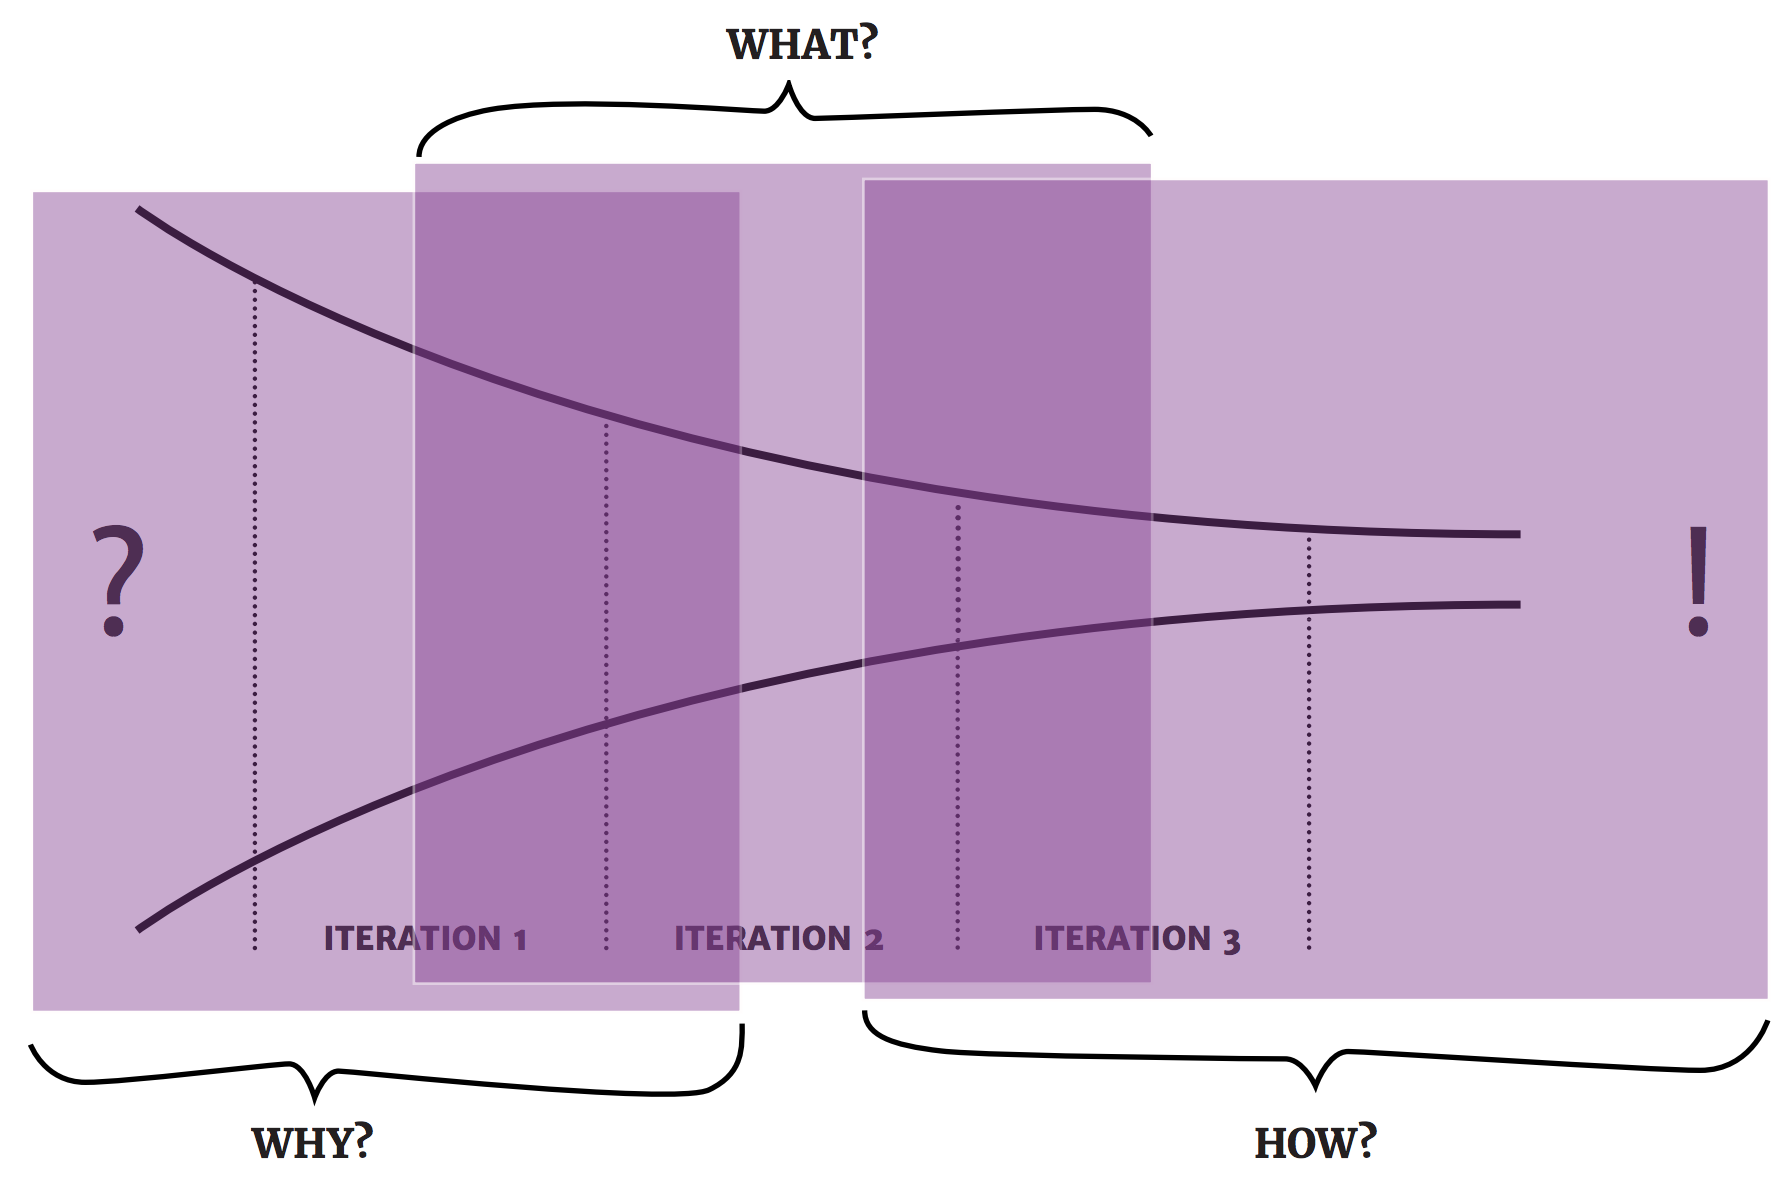
\includegraphics[width=0.25\textwidth]{IterationProcess.png}
%    \caption{Iteration process}
%    \label{fig:iterationprocess}
%\end{wrapfigure}

\begin{figure}[h]
    \centering
    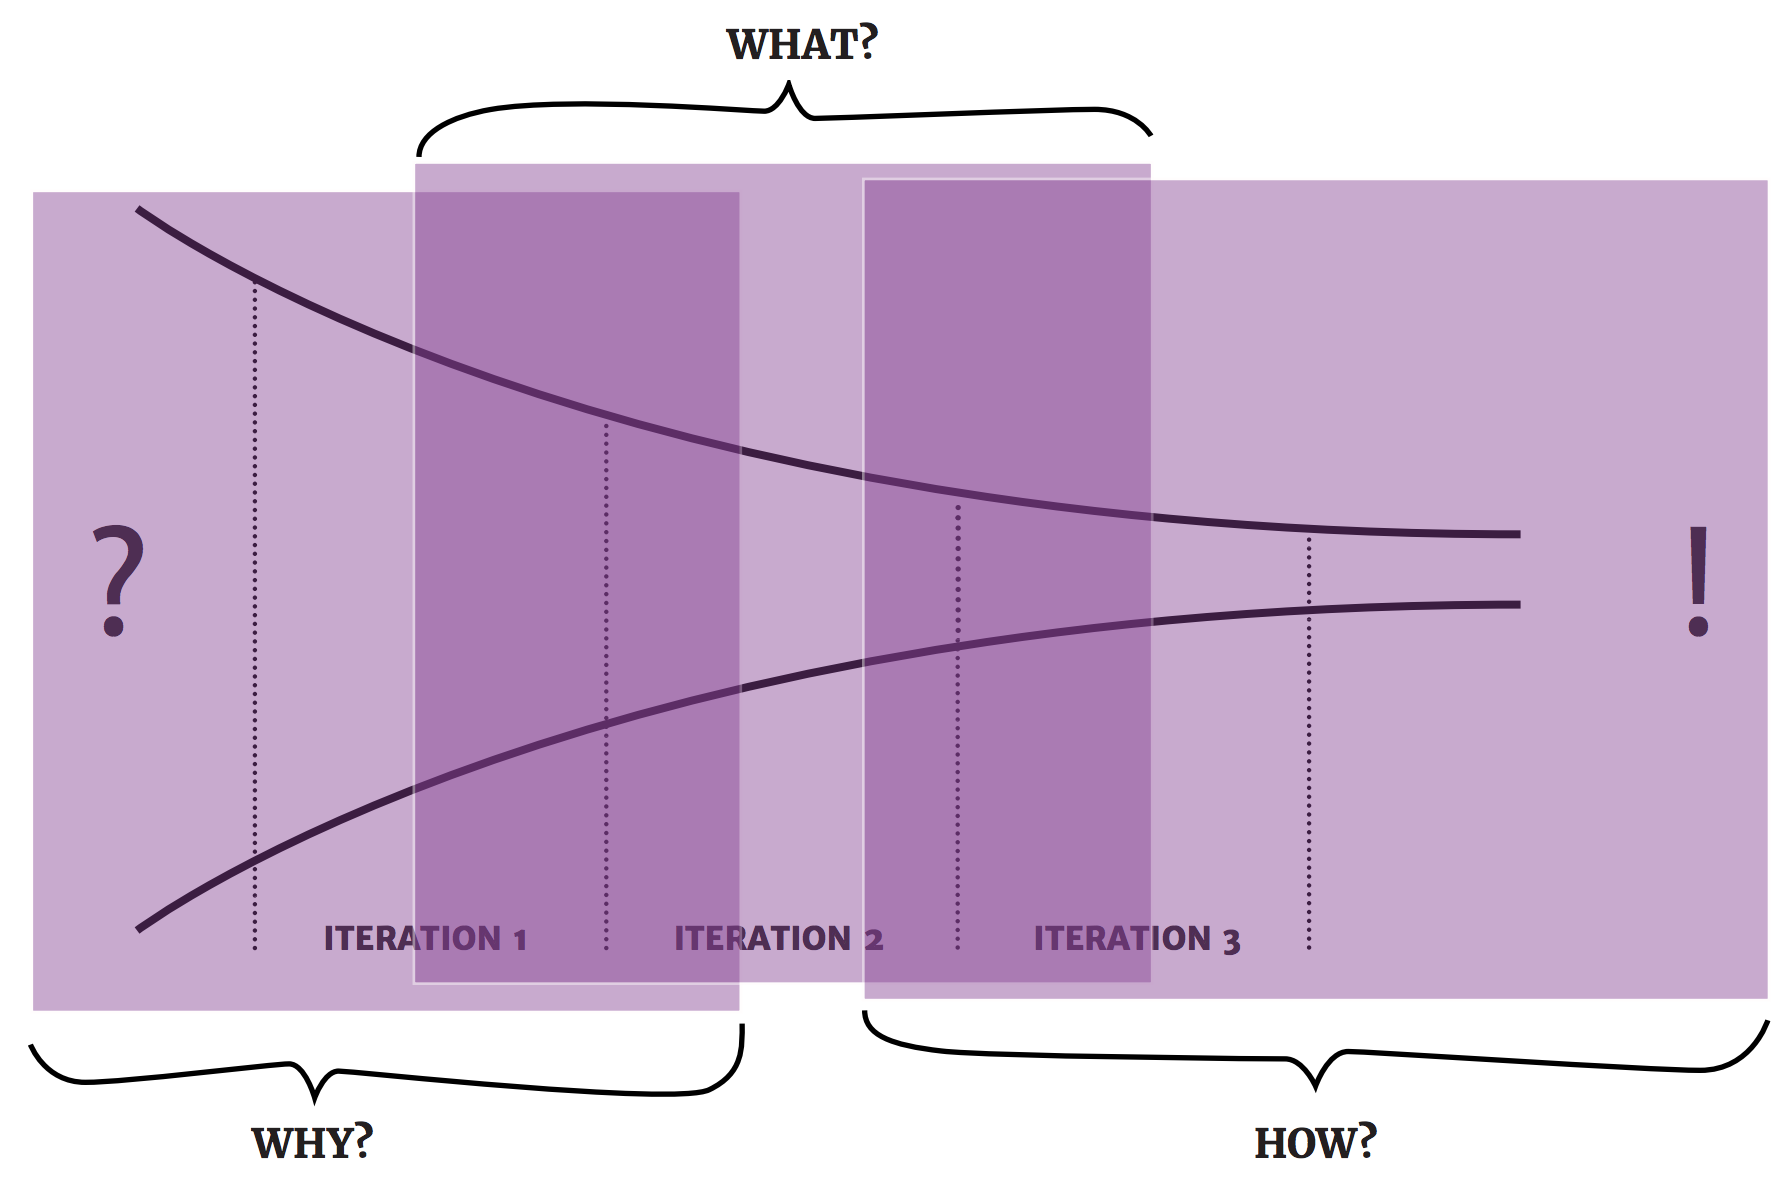
\includegraphics[width=0.8\textwidth]{IterationProcess.png}
    \caption{The iteration process consists of a number of iterations with different focus, starting with broad strokes, and narrowing down into a concrete product. Between iterations, the overlap between "Why?" and "How?", "How?" and "What?", signals that there is a learning process which means conclusions may need to be quickly questioned as new insights emerge. This is especially important in projects where you work with an unfamiliar target group and there are several uncertainties and constraints.}
    \label{fig:iterationprocess}
\end{figure}

\textbf{One iteration} \\
In the way of reasoning around development and design for learning, the steps for each iteration, see figure \ref{fig:iteration}, might be translated into:

\begin{enumerate}
\item Interactions, where you are listening, the \textit{Explorative phase}. 
\item Insights, which is where you use the Interactions in order to try to understand, the \textit{Understanding phase}. % better word+
\item Ideation, where you find possible ideas and when creation of new version of the app is done, the \textit{Design phase}.
\item Trigger material, where material is developed to test the outcome of our evaluation in the next round, the \textit{Trigger development}.
\end{enumerate}